\documentclass[11pt,letterpaper]{article}
\usepackage[margin=0.75in]{geometry}
\usepackage[latin1]{inputenc}
\usepackage{amsmath}
\usepackage{amsfonts}
\usepackage{amssymb}
\usepackage{graphicx}
\usepackage{wrapfig}
\usepackage{color}
\usepackage{caption}
\usepackage{subcaption}
\usepackage[colorlinks=false]{hyperref}
\graphicspath{{./images/}{IR}}
\usepackage{fancyhdr}
\pagestyle{fancy}
\fancyhead{}
\lhead{CS410}
\chead{Project 2 Report}
\rhead{Justin Haupt}
\author{Justin Haupt}
\title{Moving Object Detection and Tracking\\CS410 Introduction to Visual Computing\\ Winter 2017}
\date{}

\begin{document}
	\maketitle

    \newpage
	\section*{Abstract}
	It has been an ongoing problem to detect and track moving objects from video footage, and there have been many methods developed to accomplish this with varying levels of success. This report details an iOS application that features several of those methods of detection and tracking in real-time. In real-time, it is a challenge to have minimal impact on hardware resources in order to prevent lag between video frames. This app was able to significantly reduce processing time by employing two efficient algorithms, compressive tracking and background subtraction, where the performance of each tracking type experienced little to no lag. The background subtraction technique, however, detected almost all movements including some undesired lighting changes, and sometimes could not detect swathes of colors due to the camouflage effect.\\
	
	\section{Introduction}
	A video is a sequence of individual frames, and each frame contains abstractions that could potentially represent objects of interest. It is significantly more difficult for a machine to perceive what us humans can, for we don't have to think twice or develop a model of our surroundings to know which events are taking place. It is the task of detection software to sort through low-level features/pixels of an image and connect them to high-level abstractions, including motion events. Any algorithm will face the challenge of occlusion, motion blur, lighting changes, and fickle users (in a phone app). Although this subject has been studied for dozens of years, it is still a problem that has yet to attain a highly robust, and accurate solution.
	
	Object detection in video surveillance has many practical uses in business, analytics, and security. Automating such systems could gauge the flux of pedestrians and traffic, locate high-profile criminals, and even replace systems that require human oversight. Consider recent events with the advent of self-driving cars. If the market for these types of cars are about to reach average consumers in the near future, then object detection systems will have set global benchmarks in transportation safety. The following paper outlines effective methods of object detection and tracking, and how they are incorporated into a simple phone application.\\
	
	\newpage
	\section{Design}
	The main controller for this app is coded in Swift, and it uses a wrapper to access the frame processor and video source controller in Objective-C++. The foundation for this project was a repository on Github named {\tt MinimumOpenCVLiveCamera}, created by Akira Iwaya, which provided the source code for accessing an iPhone's camera with the video source controller and directing individual frames to the frame processing unit.
	
	The user interface for the app is minimal, consisting of three buttons: {\tt start}, {\tt stop}, and {\tt mode}. The {\tt start} and {\tt stop} buttons begin or pause the camera and processing of images on the screen, and the {\tt mode} button raises an alert message that provides options for mode selection.\\
	
	\noindent Available modes are selectable in the alert box:
	
	\begin{figure}[h!]
		\centering
		\begin{subfigure}{.4\textwidth}
			\centering
			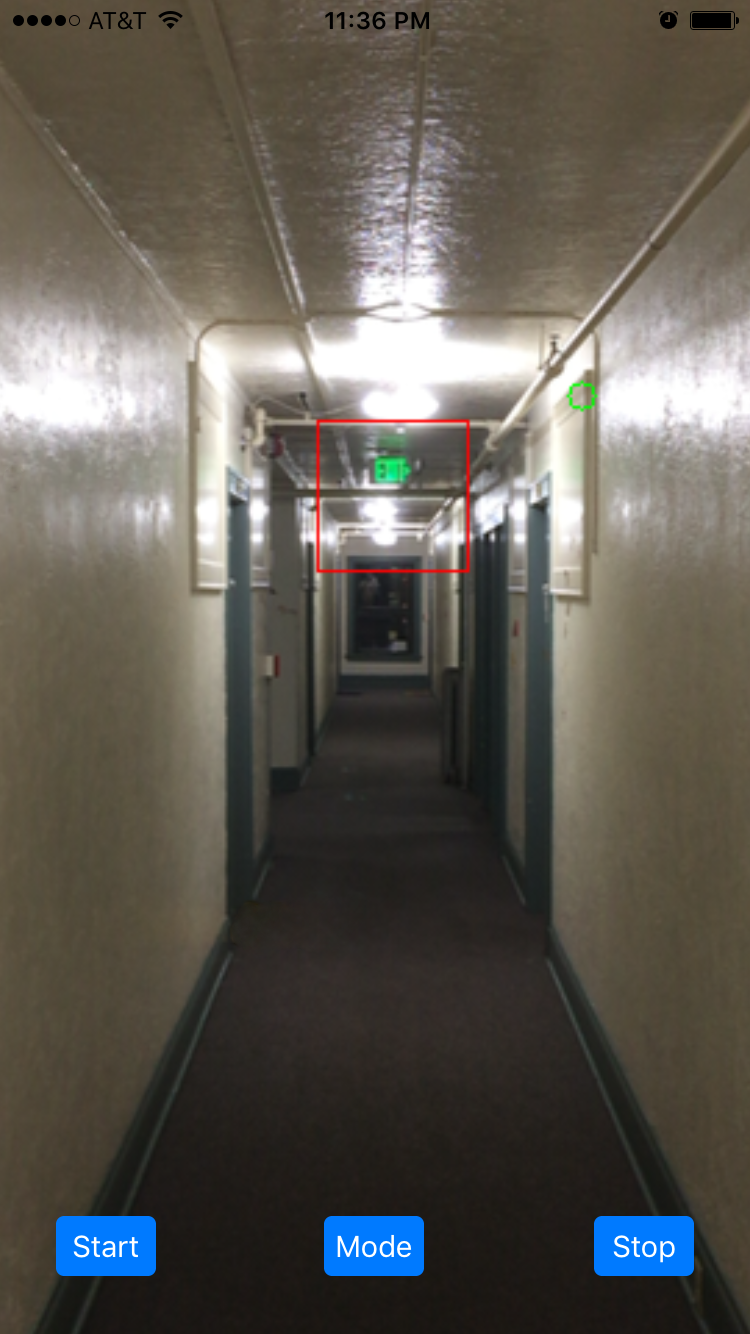
\includegraphics[width=1\linewidth]{hallway}
			\caption{main camera view}
		\end{subfigure}\space\space\space\space%    
		\begin{subfigure}{.4\textwidth}
			\centering
			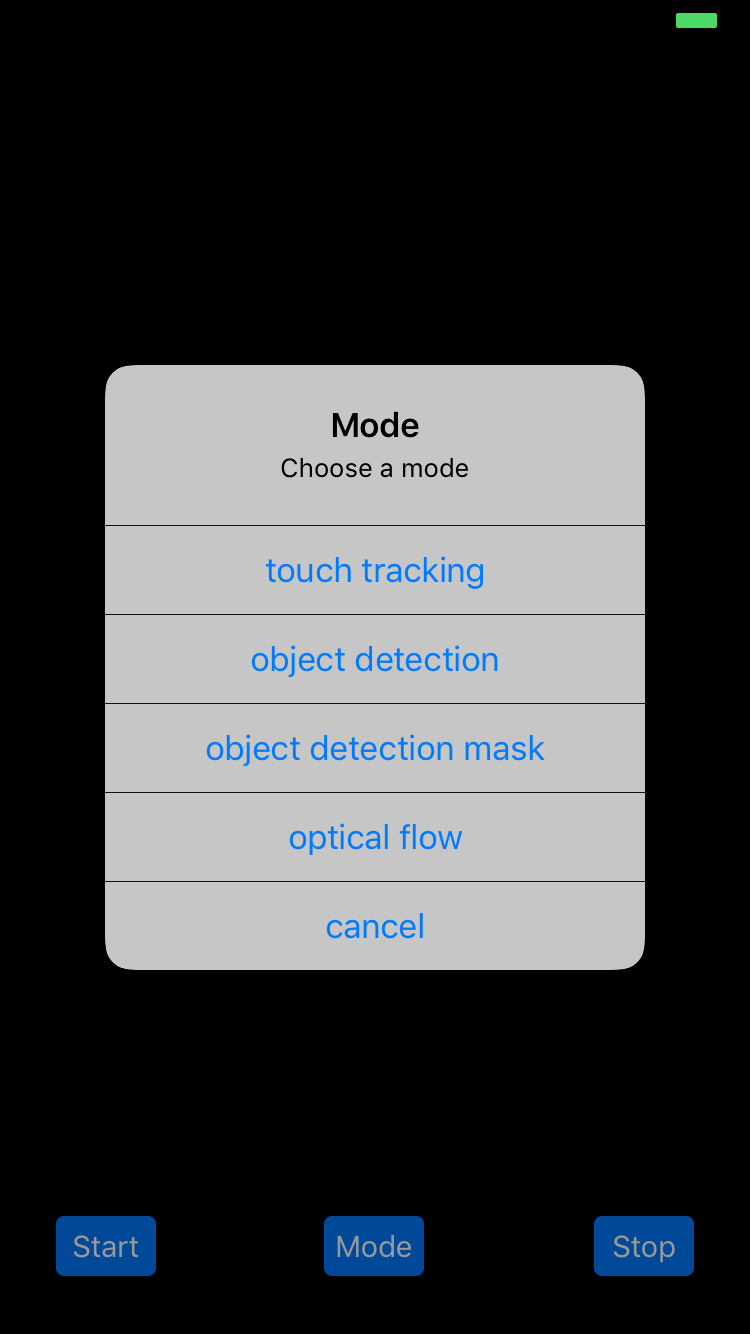
\includegraphics[width=1\linewidth]{alert_menu}
			\caption{alert menu}
		\end{subfigure}
	    \caption{User Interface}
	\end{figure}
	
	
	\newpage
	\section{Implementation}
	
	\subsection*{Compressive Tracking}
	This form of tracking was designed by a team of computer vision researchers who were determined to improve the standards and robustness of object tracking, and it was a well-founded solution for the touch tracking mode. In summary, it extracts a small amount of samples from the target window and the background area in each frame.  Then it extracts good features from each sample into a sparse matrix; several of those compressed vectors are used to update parameters of a naive Bayes classifier and to predict where the object will appear in the next frame [3].
	
	This algorithm requires that the tracking box be initialized before processing; the iOS interface allows the user to touch or slide the desired location of the tracking box onto a device's screen, where it should appear to instantaneously relocate. \\
	
	\subsection*{Background Subtraction}
	The other algorithm that was used involved background subtraction, which was used for both object detection and tracking simultaneously. This method identifies foreground objects by maintaining a background model and a mask that are updated with each frame. The mask is derived from the frame difference between the original frame and the background model, which is above some threshold value. Although this app is not intended for long hours of surveillance, the background model should theoretically update over time; so if a car enters the scene and parks there for a month, it should eventually become a part of the background. 
	
	OpenCV includes background subtraction objects. The MOG2 object was used instead of MOG because it captured more details and complete image figures with less pixel gaps. \\
	
	Here is my proposed algorithm:
	
	 \begin{enumerate}
	 	\item Apply a slight blur to the original frame
	 	\item Update the foreground mask and background model
	 	\item Reduce the resolution of the mask to approximately 1/6th of the original dimensions
	 	\item Find and reserve locations of all contours in the mask
	 	\item Approximate each contour to a polygon and store a vector of bounding rectangles
	 	\item Group all bounding rectangles that overlap one another
	 	\item Draw the bounding rectangles on the original frame that have an area larger than a pre-determined constant size
	 \end{enumerate}
	
	The light blur is applied first because it helps to reduce unwanted noise before further processing. The reducing of the mask's resolution was intended to further reduce unwanted noise and to make fine-grained mask objects more coarse-grained, which helps unify detected objects. It is still possible to have gaps from within detected objects, so the grouping of rectangles eliminates all overlapping bounding boxes.
    
    
    \newpage
	\section{Testing}
	
	Since this project is about video processing, the following images do not fully represent the demo results. Links to the demo videos can be found in the project's {\tt README} file.
	
	\subsection*{Touch Mode}
	The test for this mode utilized a free-rolling ping pong ball on a smooth surface. The tracking window is expected to remain locked onto any object that is touched.  \\
	
	\begin{figure}[h!]
		\centering
		\begin{subfigure}{.4\textwidth}
			\centering
			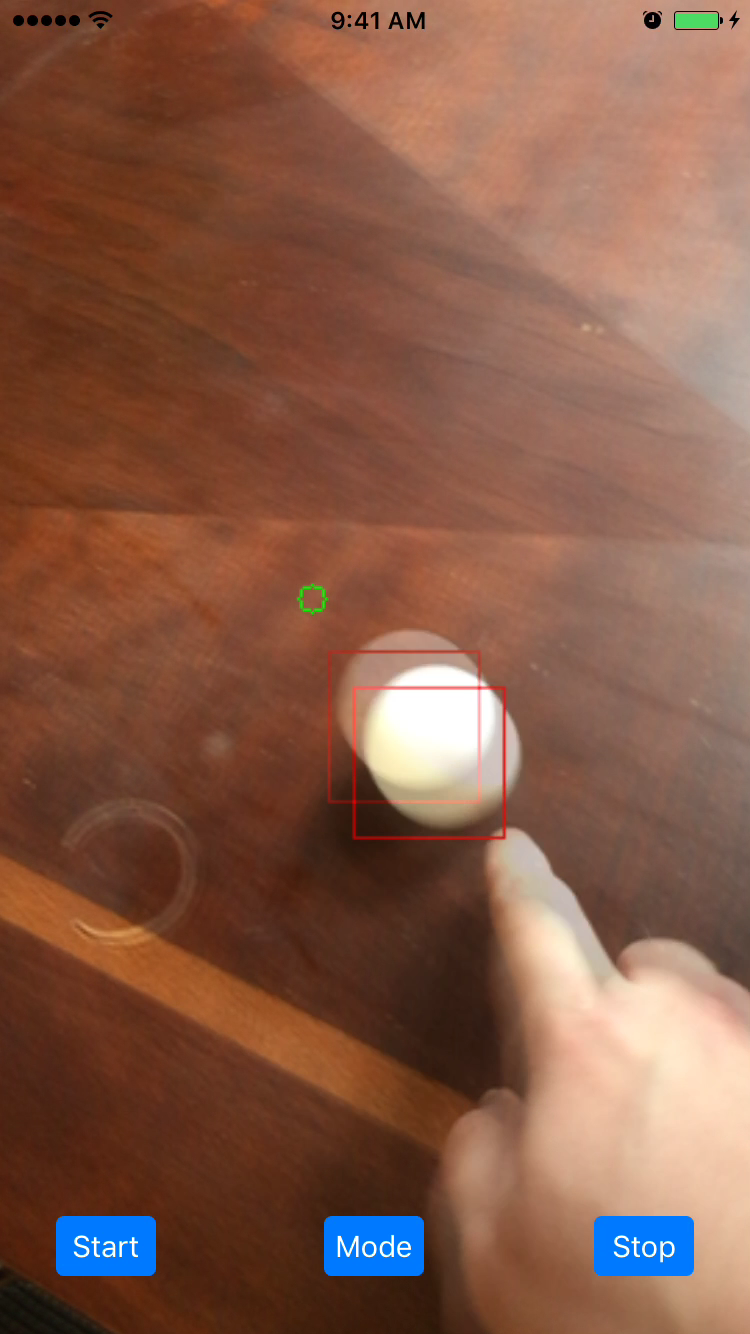
\includegraphics[width=1\linewidth]{toucha}
		\end{subfigure}\space\space\space\space%    
		\begin{subfigure}{.4\textwidth}
			\centering
			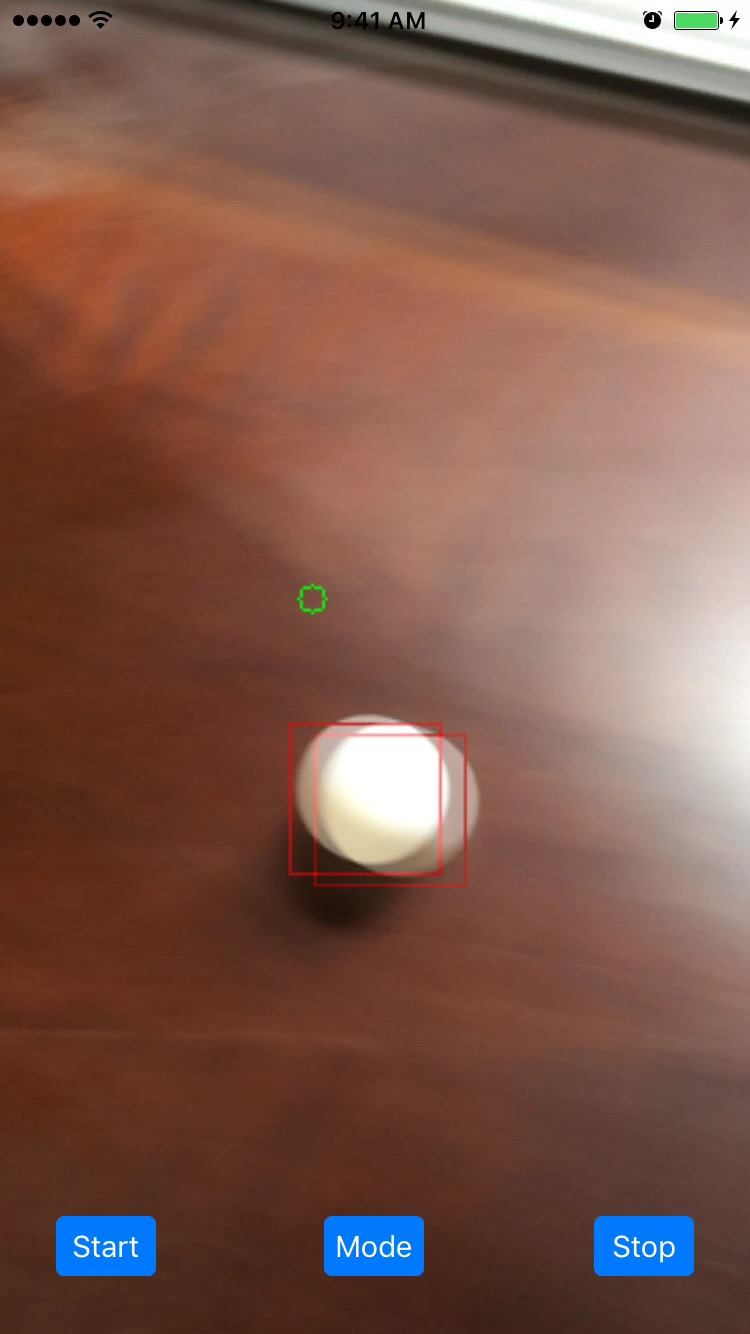
\includegraphics[width=1\linewidth]{touchb}
		\end{subfigure}
		\caption{Compressive tracking movement}
	\end{figure}

    Upon touching the ping pong ball on the phone's screen, the tracking box is relocated on the ball and follows its movements. At one point in the video, the ball exits the edge of the frame, and the tracking window simply locks onto something else; then the ball is touched for a second time and the window relocates back onto the ball.
	
	\newpage
	\subsection*{Object Detection}
	This test for the background subtraction method was conducted at a traffic intersection, in view of pedestrians and vehicles. \\
	
	\begin{figure}[h!]
		\centering
		\begin{subfigure}{.4\textwidth}
			\centering
			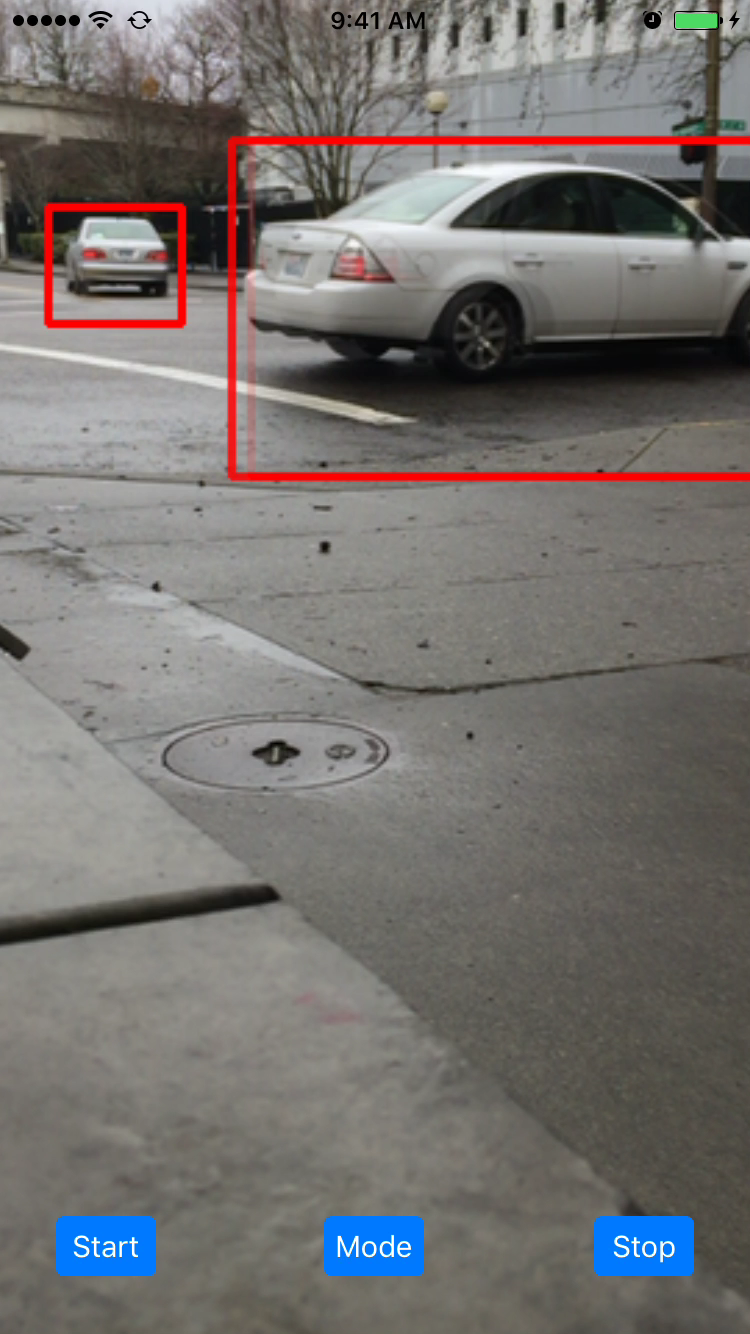
\includegraphics[width=1\linewidth]{mode2a}
		\end{subfigure}\space\space\space\space%    
		\begin{subfigure}{.4\textwidth}
			\centering
			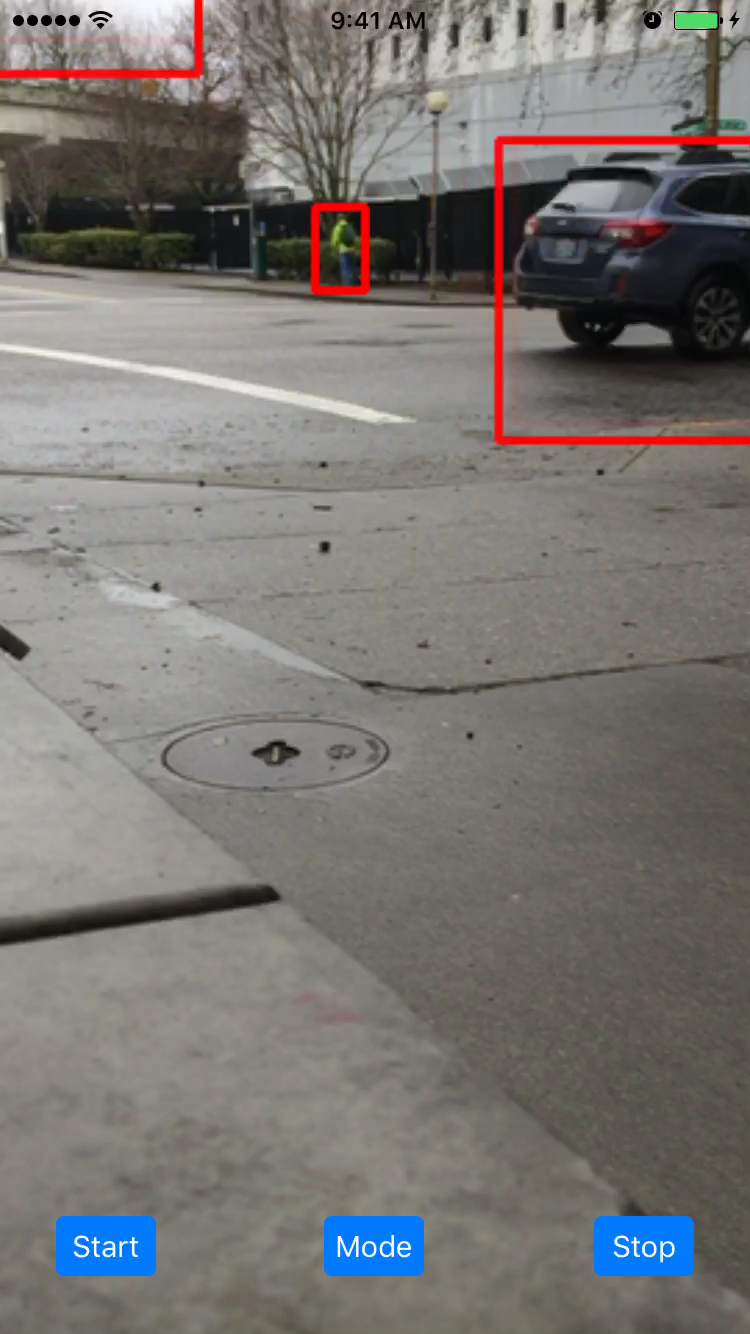
\includegraphics[width=1\linewidth]{mode2b}
		\end{subfigure}
		\caption{Compressive tracking movement}
	\end{figure}

    It was a damp and rainy day, so the detector identified clouds and reflections on the concrete as moving objects. In addition, people who wore black jackets blended in with the large black fence in the background, so their torsos were not identified. Despite this undesired behavior, all vehicles on the road were completely identified and tracked.
	
	\newpage
	\subsection*{Object Detection Mask}
	This test is the same as the previous test, except the mask is observed. \\
	
	\begin{figure}[h!]
		\centering
		\begin{subfigure}{.4\textwidth}
			\centering
			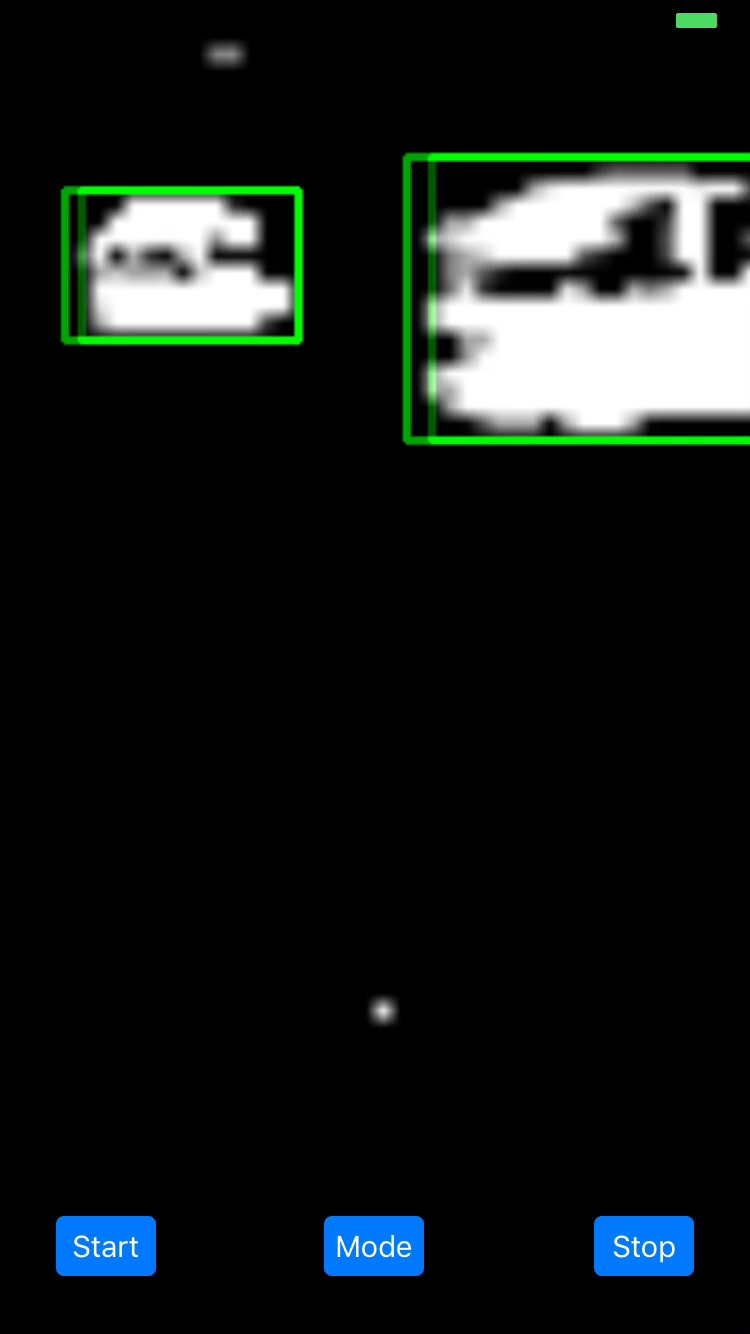
\includegraphics[width=1\linewidth]{mode3a}
		\end{subfigure}\space\space\space\space%    
		\begin{subfigure}{.4\textwidth}
			\centering
			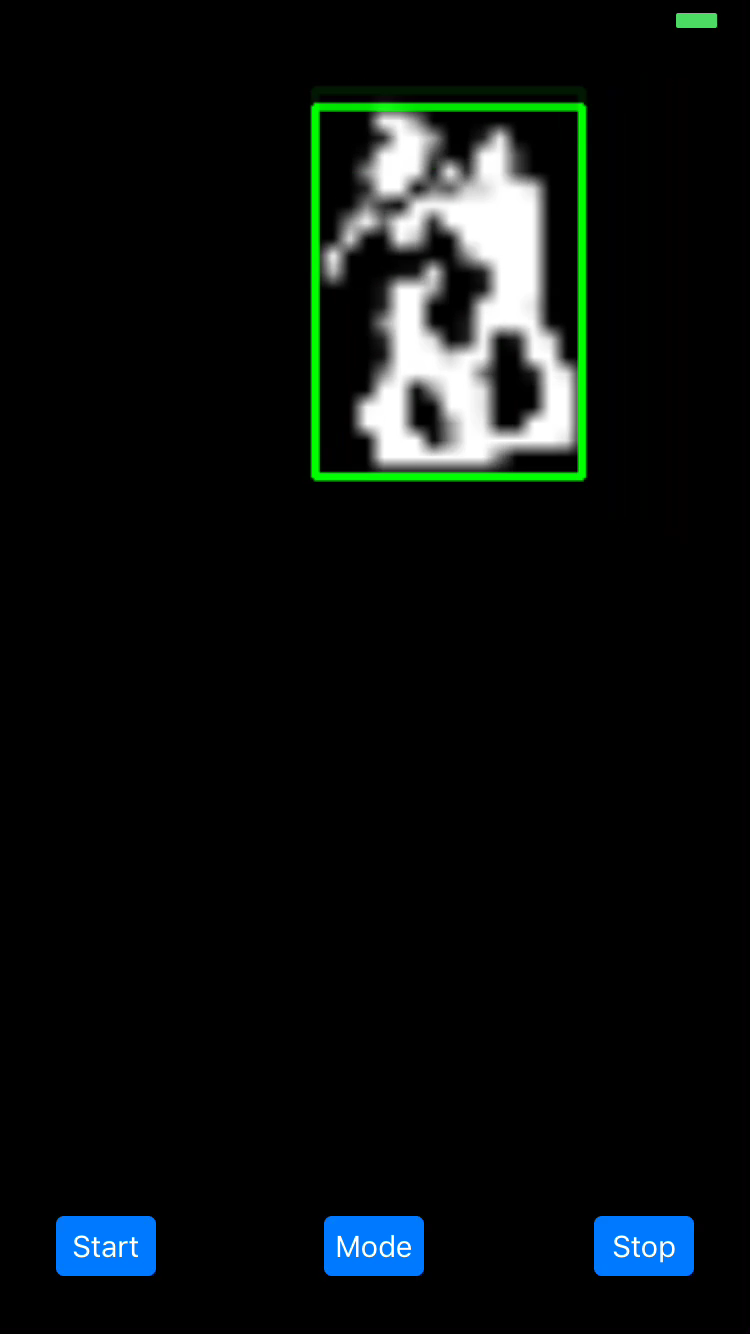
\includegraphics[width=1\linewidth]{mode3b}
		\end{subfigure}
		\caption{Compressive tracking movement}
	\end{figure}

    In this video, there was an instance where the bounding box of one of the vehicles briefly fragmented into several parts, and was mostly caused by the shadow. This could have been avoided with some form of shadow removal or increased mask simplification.

	
	\newpage
	\begin{thebibliography}{9}
		
		\bibitem{abouttracking1} 
		Porikli, F., and A. Yilmaz. Object Detection \& Tracking. Publication. MITSUBISHI ELECTRIC RESEARCH LABORATORIES, Jan. 2012. Web. 15 Mar. 2017.\\ \url{https://pdfs.semanticscholar.org/afa0/3ff6c32142ae9ae1651fc4850bf8d3d8c228.pdf}
		
		\bibitem{abouttracking2}
		Guo, Zhong. "Object Detection and Tracking in Video." Department of Computer Science, Kent State University, Nov. 2001. Web. 15 Mar. 2017.\\ \url{http://medianet.kent.edu/surveys/IAD01F-objdetection/index.html}
		
		\bibitem{compressivetracking}
		Zhang, Kaihua, Lei Zhang, and Ming-Hsuan Yang. Real-Time Compressive Tracking. Publication no. 7574. Berlin Heidelberg: Springer-Verlag, 2012. Print.\\
		\url{http://www4.comp.polyu.edu.hk/~cslzhang/CT/CT.htm}
		
		\bibitem{backgroundsubtraction}
		Tamersoy, Birgi. "Background Subtraction." Texas, Austin. 29 Sept. 2009. Web. 15 Mar. 2017.\\ \url{http://www.cs.utexas.edu/~grauman/courses/fall2009/slides/lecture9\_background.pdf}
	\end{thebibliography}
	
	

\end{document}